\section{Analysis of the problem and variables identification}
\subsection{Scope of the problem}
To approach the problem of this article, it is necessary to understand how the dynamic of buying and selling coins through the exchanges can affect the price of that specific cryptocurrency; at the same time, it is important to notice how goverment regulation can affect the price, so we can thoroughly determine how effective will goverment taxes affect the system.

\subsection{Model purpose}
Understand how the cryptocurrency buying-selling dynamic through exchanges, can increase growth rate and affect the price altogether. Therefore, understanding how fraudelent schemes can leverage this system exponentially and artificially manipulate the price.

\subsection{Variables identification and historical background}
We identified 10 variables that affect the problem of over inflating this types of currencies for scams. These are:
\begin{enumerate}
	\item Price of the cryptocurrency (CC): this is the market value in US dollars that the actual coin has. Measurement units: \$ USD
    \item Number of CC bought: is the number of CC bought by the users through the Exchanges. Measurement units: dimensionless.
    \item Number of CC sold: is the number of CC sold by the users to the Exchange company for another currency. Measurement units: Dimensionless.
    \item Investors: is the number of investors that have invested on the coin or the company releasing it. Measurement units: dimensionless.
    \item Number of Exchanges: this is the number of Exchanges that trade this specific CC. Measurement units: dimensionless.
   	\item Volatility: it's the uncertainty in percentage of, given a value of winning fee, how much one can lose or win in relation to that fee. Measurement units: \%
    \item Earnings: this is on average how much a given person earns by trading this CC. Measurement units: \$ USD
    \item Exchange fees: this is the fee that the Exchange uses in every trade you make with their rates. Measurement units: \$ USD
    \item Government taxes: this is the taxes that the government applies to the Exchange. Measurement units: \$ USD
    \item Growth rate: It refers to the price of the cryptocurrency divided by time\cite{GR}. Measurement units: USD/Time.
\end{enumerate}

\noindent In order to give some historical background of these variables, we are going to use the BitConnect example because, although there exists several companies who work in a similar fashion, this is the only one in this span of time that has completed the scam completely. It is important to notice that, finding measurements of variables such as the CC sold and bought can be a real hard task because the number of transactions per day with this coin considerably big; and, although we could check the blockchain for every single operation in each CC, it is something to improve upon in the future with an algorithm that does this automatically.

\noindent In this manner, instead of measuring the CC sold and bought will find the historical background of the Volume of the CC which represents the amount of money in USD that has been traded of that CC every 24 hours; even if is not exactly the same as the variables mentioned, we could have a good knowledge of this variables through that graph. Figure \ref{img-trading} shows trading data on BitConnect.
\begin{figure}[H]
	\centering
    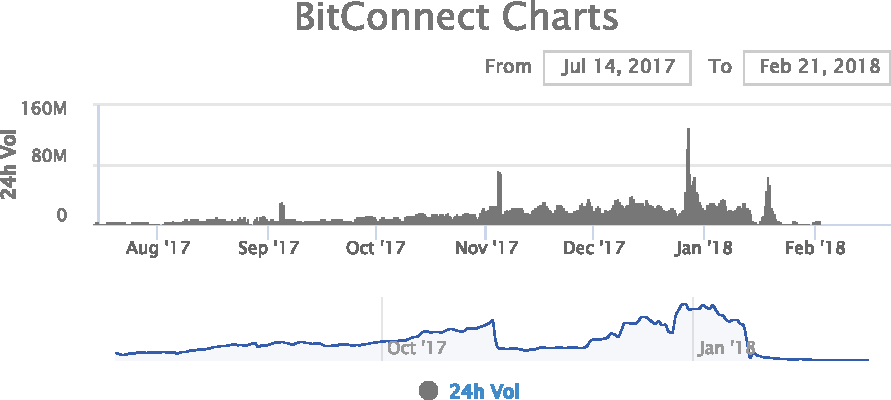
\includegraphics[scale=0.8]{files/Trading.pdf}
    \caption{Trading data on BitConnect.}
    \label{img-trading}
\end{figure}

\noindent On the other hand, the same occurs when we try to find the number of investors; it would be something impossible to find at exact quantity of how much investors are investing in the CC. So, instead, we can find the graph of the Market Cap that is the number of investors multiplied the price of a unitary action of the company. In this way, we would get a very good grasp of the behavior of this variable. Figure \ref{img-marketcap} shows said data.

\begin{figure}[H]
	\centering
    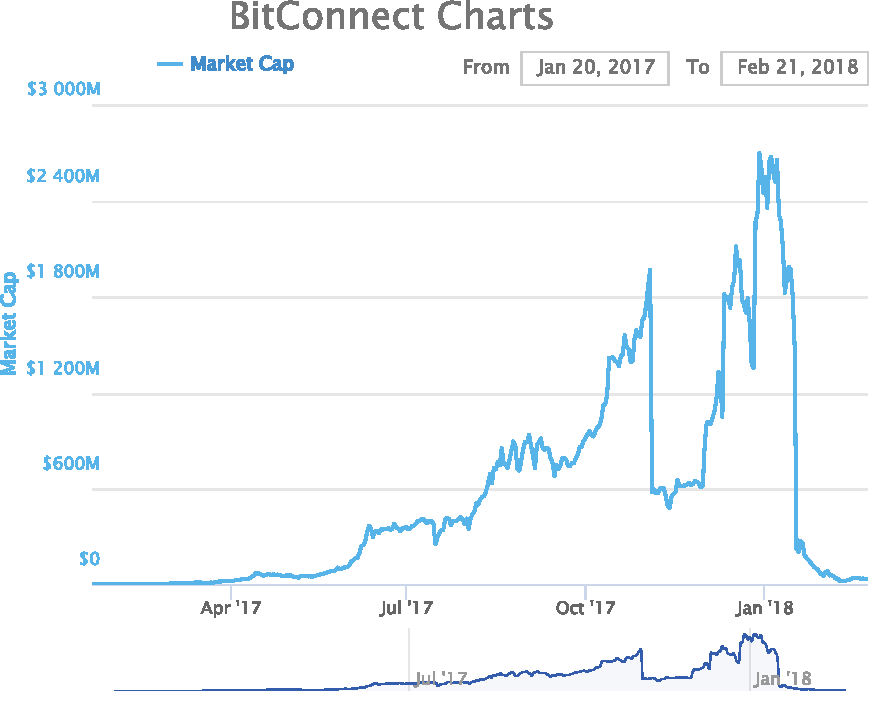
\includegraphics[scale=0.7]{files/Market_Cap.pdf}
    \caption{Market cap data on BitConnect.}
    \label{img-marketcap}
\end{figure}

\noindent Finally, the price of the CC is the easiest to find, as it is documented in a wide variety of websites. Figure \ref{img-pricebcc} shows the price of the BitConnect Coin.

\begin{figure}[H]
	\centering
    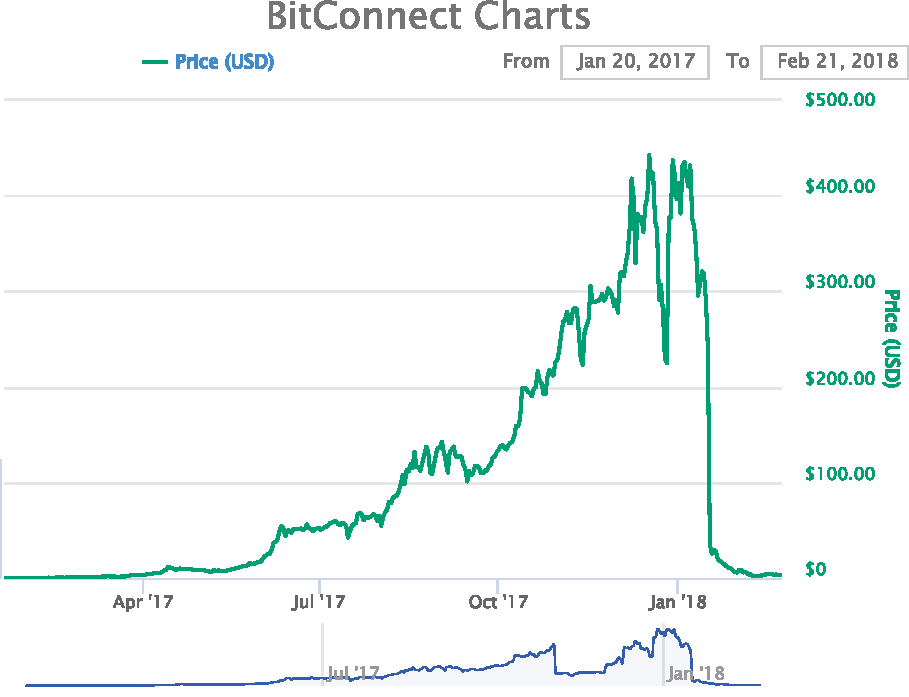
\includegraphics[scale=0.7]{files/Price_bCC.pdf}
    \caption{Price on BitConnect Coin.}
    \label{img-pricebcc}
\end{figure}

This data was obtained from Coin Market Cap on \cite{cmc}.
